% ---------------------------------------------------------------------------
% Figure captions, ready to paste. graphicx is already loaded in extra_pkgs.tex.
% neurips.sty is single-column article with textwidth=5.5in, so these are
% ordinary `figure` floats -- NOT figure*. The PDFs are authored at 5.5in, so
% \includegraphics[width=\textwidth] places them 1:1 and the point sizes in the
% figure are the point sizes on the page.
% Add to the preamble if not present:  \graphicspath{{figures/}}
%
% Placement (see figures/README.md for the reasoning):
% NOTE: paper/Makefile sets FIGURES_FOLDER := figures and runs pdfcrop over
% paper/figures/*.pdf. The figures live one level up, at NeurIPS_workshop/figures.
% Either symlink (ln -s ../figures paper/figures) or point \graphicspath there.
%
%   Fig 2  -> \section{What form do the shortcuts take?}  (sec:forms, l.199),
%             at the top of the page carrying "Not every corpus has the same
%             shortcut" (l.369). It is the figure that paragraph argues from.
%   Fig 3  -> \subsection{Inside the model...}  (sec:probing, l.288), top of the
%             page holding "The contamination is total" (l.305) and "And the
%             part that does vary does not explain behaviour" (l.336) -- panel
%             (a) is the first, panel (b) is the second.
%   Fig 4  -> \section{Mitigation} (sec:mitigate, l.395), after Table 2
%             (tab:mitigate). Fig 4 is the per-model view of the row that table
%             aggregates, so it must follow, not precede it.
%
% NOTE: Fig 3's caption previously cited Appendix~\ref{app:probing} for the
% other three models' random-direction controls. No such appendix exists yet.
% Either add one (the arrays are in
% experiments/i7-causal-probing/results/layerwise_multi.json) and restore the
% cross-reference, or leave the wording as it stands.
% ---------------------------------------------------------------------------

\begin{figure}[t]
  \centering
  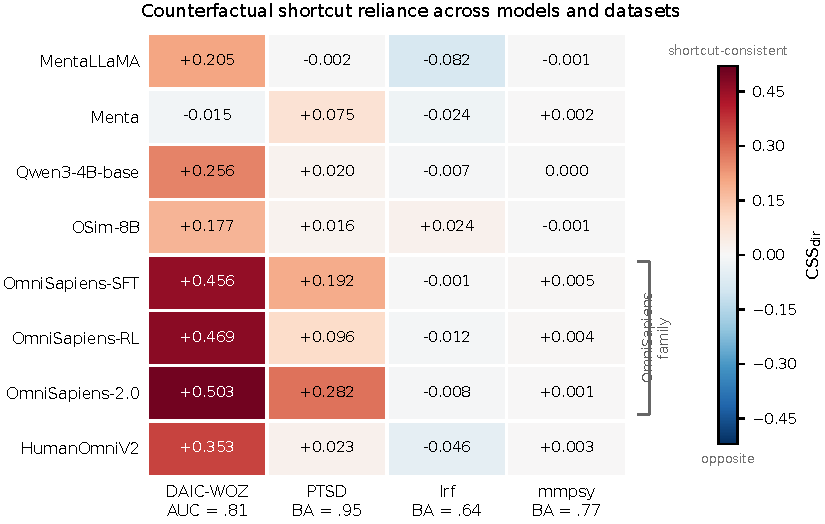
\includegraphics[width=\textwidth]{figures/figure2_css_heatmap.pdf}
  \caption{\textbf{A statistically available shortcut is not a shortcut the
  model uses.} Directional counterfactual shortcut sensitivity
  ($\mathrm{CSS}_{\mathrm{dir}}$, the mean paired change in predicted
  probability when only the shortcut-bearing content is swapped and the item's
  own content is held byte-identical) for eight models on four corpora
  ($n=188$, $60$, $400$, $190$). Colour is symmetric about zero so that
  intensity is comparable across the sign; exact values appear in every cell.
  DAIC-WOZ moves all eight models; PTSD moves mainly the OmniSapiens family;
  Irf is weak and, on four models, reversed; mmpsy is null throughout despite
  carrying the second-strongest data-level signal in the panel. The probe
  metrics under each column index whether a shortcut is \emph{statistically
  available} in that corpus; they use different tasks and different metrics and
  \textbf{are not comparable to one another}.}
  \label{fig:css-heatmap}
\end{figure}

\begin{figure}[t]
  \centering
  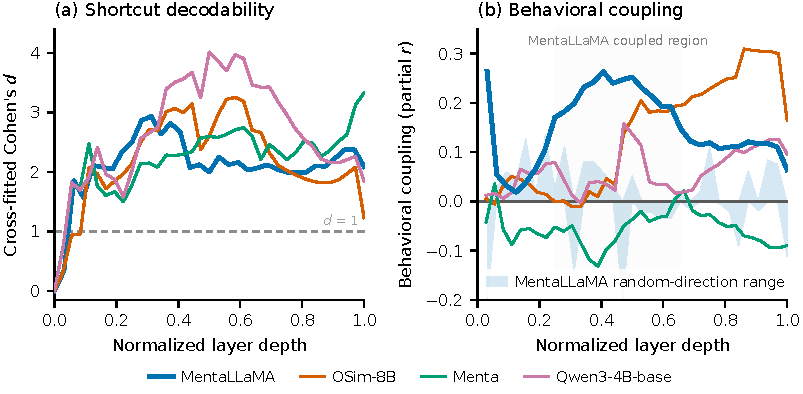
\includegraphics[width=\textwidth]{figures/figure3_layerwise.pdf}
  \caption{\textbf{The shortcut is decodable almost everywhere and
  behaviourally relevant almost nowhere.} \textbf{(a)} Cross-fitted linear
  separation between clinically loaded and biographical interviewer contexts,
  measured on held-out folds with grouping by participant. It exceeds $d=1$ at
  $89$--$95\,\%$ of layers in all four models (peaks $2.93$--$4.01$); the
  shuffled-label control reaches at most $0.24$. \textbf{(b)} Partial
  correlation between movement along the learned shortcut direction and the
  per-participant shift in prediction, controlling for the norm of the
  representational displacement. The shaded band is MentaLLaMA's \emph{own}
  matched random-direction range. Only MentaLLaMA's learned direction leaves
  its control, over a contiguous span of layers ($15/32$ layers significant,
  random winning on $5$). For the other three, a random direction wins on
  $15/36$, $18/36$ and $21/36$ layers; their controls are omitted
  here for legibility. The two quantities are on separate axes because
  their dissociation is the claim.}
  \label{fig:layerwise}
\end{figure}

\begin{figure}[t]
  \centering
  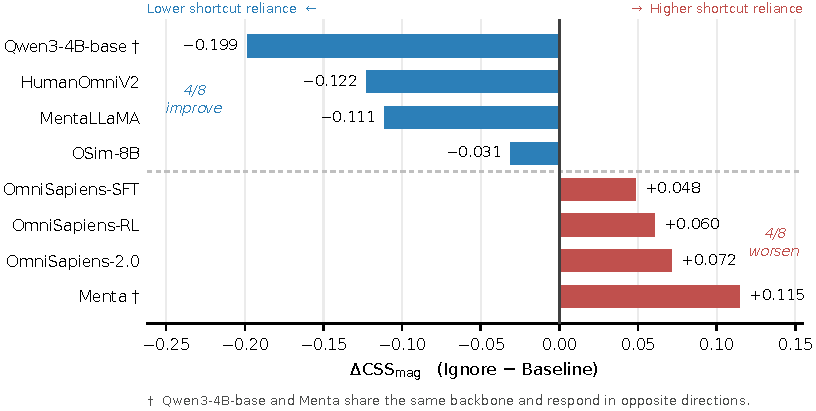
\includegraphics[width=\textwidth]{figures/figure4_mitigation_heterogeneity.pdf}
  \caption{\textbf{One mitigation, opposite effects.} Change in shortcut
  sensitivity after adding an instruction to ignore the interviewer, across the
  eight-model DAIC-WOZ sweep. Negative is a reduction. Exactly four models
  improve and four worsen, so the aggregate in Table~\ref{tab:mitigate}
  averages over a sign change rather than over noise. Qwen3-4B-base and Menta
  ($\dagger$) share a backbone and respond in opposite directions
  ($0.256 \to 0.058$ against $0.027 \to 0.141$), which rules out model scale or
  architecture as the explanation. We plot this method because it is the only
  arm in the shared sweep whose post-intervention CSS is \emph{measured};
  deleting, masking or marginalising the channel drives CSS to zero by
  construction, since nothing is then left to swap.}
  \label{fig:mitigation-heterogeneity}
\end{figure}
